\documentclass[12pt,a4paper]{article}
\usepackage[latin2]{inputenc}
\usepackage{graphicx}
\usepackage{ulem}
\usepackage{amsmath}
\usepackage[margin=0.5in]{geometry}
\usepackage[T1]{fontenc}
\usepackage[ampersand]{easylist}
\usepackage[english]{babel}
\usepackage{scrextend}
\usepackage{subfig}
\usepackage{float}
\usepackage{stackengine}
%\usepackage[demo]{graphicx}
%\usepackage{caption}
%\usepackage{subcaption}
%\usepackage[utf8]{inputenc}
\begin{document}

%%%%%%%%%%%%%%%%%%%%%%%%%%%%%%%%%%%%%%%%%%%%%%%%%%%%%%%%%%%%%%%%%%%%%%%%%%%%%%%%
% Document Setup

\pagenumbering{arabic}
\setcounter{page}{0}

%%%%%%%%%%%%%%%%%%%%%%%%%%%%%%%%%%%%%%%%%%%%%%%%%%%%%%%%%%%%%%%%%%%%%%%%%%%%%%%%
% Title block - Page 0

% Cover page. Clearly indicate the names of the team members.
% Also provide a table comparing the given specs and achieved spec (remember
% this is for the NON-BONUS part of the project only). You also need to provide
% us a percentage-wise break down of area consumed by different sections of
% bias circuit (VNMOS-bias, VPMOS-bias & bias generator circuit) as compared to
% your core circuit area (refer to Figure 3). For area calculation, use
% AMOS = W * L. Also include the area of resistors in your design. Assume that
% the sheet resistance is 5.5 kohm/sq and the minimum length of resistor is
% 1 um

\author{
  Kankanala, Usha\\
  \texttt{ukankana@stanford.edu}\\
  \texttt{SUID:06091239}
  \and
  Lenius, Samuel\\
  \texttt{lenius@stanford.com}\\
  \texttt{SUID:06091240}
}

\title{2015 EE214A Design Project}

\maketitle

%%%%%%%%%%%%%%%%%%%%%%%%%%%%%%%%%%%%%%%%%%%%%%%%%%%%%%%%%%%%%%%%%%%%%%%%%%%%%%%%
% Performance Summary Block - Page 0

\begin{abstract}
  Area Breakdown:
  \begin{addmargin}[1em]{0em}
  \begin{itemize}
    \item PMOS Bias Gen: 25\%
    \item NMOS Bias Gen: 25\%
    \item Core circuit: 25\%
    \item Resistors: 25\%
  \end{itemize}
  \end{addmargin}
\end{abstract}

\pagebreak

%%%%%%%%%%%%%%%%%%%%%%%%%%%%%%%%%%%%%%%%%%%%%%%%%%%%%%%%%%%%%%%%%%%%%%%%%%%%%%%%
% Design Outline - Page 1

% Outline of your design. How did you approach this problem? What are some of
% your key design choices? Flow charts and graphs of how the trade-offs are
% connected provide the best clarity in explaining (we'll show some examples in
% class). Half of the grading (i.e. 25 Points) is related to Design Flow,
% Insight and Optimization Strategy. The clarity of your discussion and the
% insight you give, starting on Page 1, is a major factor in doing well for
% these 25 Points.

\section{Design Outline}

\paragraph
Our approach to this design was to first develop sizing ratios of the transistors and their DC relationships to Vx, Vy, Vz and Vo.
We developed the equations necessary to `program' those voltages and to develop what their reasonable ranges are.
Here are some graphs that show the relationships between the output common mode voltage and Vz, and then Vz to Vy given our sizing decisions.
We developed a MATLAB program to quickly estimate critical parameters for a given design, to allow easy investigation of parametric variation.

\begin{figure}[H]
	\footnotesize
	\stackunder[5pt]{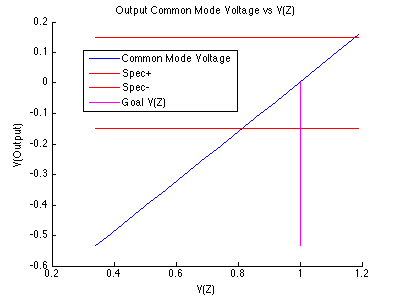
\includegraphics[width=0.4\textwidth]{cmv_vs_vz.png}}{}
	\hfill
	\stackunder[5pt]{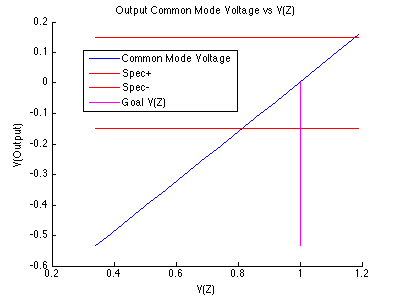
\includegraphics[width=0.4\textwidth]{cmv_vs_vz.png}}{}
\end{figure}


These graphs give rise to a process to choose exactly the value of those voltages based on the size of the transistors.
Here, given the common mode output spec, choosing a size for MN10, and estimating the MN10 backgate gives the needed value of Vz.
Given a size ratio for MN7 to MP8 gives the needed value of Vy, knowing Vz.
Given the size ratio for MP4 to MN6 and knowing the value of Vy gives the gives the necessary ratio of R3 to R4 to program the value of Vy.

\pagebreak

%%%%%%%%%%%%%%%%%%%%%%%%%%%%%%%%%%%%%%%%%%%%%%%%%%%%%%%%%%%%%%%%%%%%%%%%%%%%%%%%
% Design Schematic - Page 2

% Schematic diagram of your final design, with component values (i.e. W, L
% values etc.), node voltages and bias currents (from SPICE .op simulation)
% clearly labeled (Spend time to make this schematic complete, readable, and
% clear!). Show component values right next to the components, and currents next
% to the branches (i.e., absolutely, positively do not make us refer to a
% look-up table!). Annotate all transistors with their drain current, gate
% overdrive VOV (from SPICE .op simulation) and W/L.

\section{Design Schematic}
Text of design schematic

\pagebreak

%%%%%%%%%%%%%%%%%%%%%%%%%%%%%%%%%%%%%%%%%%%%%%%%%%%%%%%%%%%%%%%%%%%%%%%%%%%%%%%%
% Calculation of Key Design Parameters - Page 3-6

% Calculation of key design parameters, such as transconductances, bias
% currents, etc. This is the most important section of your report for giving
% critical discussion! Compare the most relevant hand calculated values with
% final SPICE values in a table and discuss discrepancies (percentage
% differences will be clear, you need to show you understand them). Make sure to
% include the total power dissipation of your design (calculated value and SPICE
% result). The lowest power designs will not automatically score the highest
% grades. The methodology you used to justify your design choices and component
% values is far more important (see section on point distribution below).

\section{Calculation of Key Design Parameters}

\textbf{Choice of L}

\begin{itemize}
\item All devices used in current source have a minimum length of 2um.
\item All other devices in the amplifier have minimum length of 1um. 
Mimimum length is used as f$_{t }$is inversely proportional to L.
\item All devices in bias generator circuit have length $>$=2um.
\end{itemize}


\textbf{Bias Generator circuit}

\begin{itemize}
\item Constant gm reference based design is used as bias circuit to 
reduce mismatch errors.
\item Transconductance of bias device (mn300) depends only on R2 and m ( 
m is the ratio of MN300/MN400). Therefore gm can be set precisely.
\item Start-up circuit is used to force the circuit to the desired 
operating point.
\end{itemize}


\textbf{Approximations for hand calculations}

For simpler hand calculations, following approximations are used.

\newcounter{numberedCntBB}
\begin{enumerate}
\item $Cdb=Csb=0.35 Cgs$
\item $Cgs=(\frac{2}{3})WLCox+Cov'W$
\item $Cgd=Cov'W$
\item $gmb=0.2gm$
\setcounter{numberedCntBB}{\theenumi}
\end{enumerate}
\textbf{Stage4}

\begin{itemize}
\item As per the spec, common mode output voltage (vout) has to be 
within -0.15v to 0.15v. Since the body is connected to vss, MN10 
experiences back gate effect and the threshold voltage is given by
\end{itemize}
$Vt=Vt0+ ?(\sqrt{2\emptyset f+Vsb}- \sqrt{2}\emptyset f$ where $
t0=0.5v$ , $?=0.6$ , $2\emptyset f=0.8$



\begin{itemize}
\item Stage 4 is a source follower which has a gain given by $
A4=\frac{gm10}{gm10+gmb10+(\frac{1}{RL})}$
\end{itemize}
Gain of stage4 (A4) $<$1 due to back gate effect and the output load. 

\newcounter{numberedCntF}
\begin{enumerate}
\item To achieve gain closer to 1 (0.6 - 0.7), it is important to size 
and bias MN10 such that (gm10+ gmb10) $>$$>$ (1/RL). 
\begin{itemize}
\item Transconductance of gm10 is given by $gm10= \mu 
nCox(\frac{W}{L})Vov10$
\end{itemize}
\end{enumerate}
Drain current $Id10=0.5\mu nCox(\frac{W10}{L10})Vov10^{2} (1+\lambda 
(Vdd-Vout)$

\begin{itemize}
\item MN9 (bias device for source follower) is sized such that I$_{d10 
}$+ I$_{RL }$= I$_{d9 }$and the common mode output voltage does 
not fall out of range. This device is chosen to be of smaller size to 
reduce loading on Vout node. 
\item $\tau stage4 (at Vout)=(RL || 
(\frac{1}{1.2gm10}))(CL+Csb10+Cgd9+Cdb9)$
\end{itemize}
Cgs10 is assumed to be very small due to boot-strapping.



\textbf{Stage 3}



\begin{itemize}
\item Loading at node Vy increases with the increase in gain of stage 3 
due to miller effect. Hence gain of stage3 is kept low and is fixed at 
sqrt(2) to compensate for the gain lost in stage 4. 
\end{itemize}
Gain of stage3 (CS amplifier with diode connected load)



$
abs(A3)=\frac{gm7}{gm8}=\frac{Vov8}{Vov7}=\frac{Vdd-Vz-abs(Vtp)}{Vy-Vss-Vtn}= 
\sqrt{2}$\\


 

Choice of Vz from above (stage4) determines Vy.

\begin{itemize}
\item Minimum device sizes (W=2um, L=1um) are used for both MN7 and MP8 
to reduce loading on Vy and Vz.
\end{itemize}
Drain current $Id7=Id8=0.5\mu nCox(\frac{W7}{L7})Vov7^{2} (1+\lambda 
(Vz-Vss)$

\begin{itemize}
\item $\tau stage3 (at Vz)=(\frac{1}{gm8})(Cgs8+Cdb8+Cgd10+Cgd7 
(1+\frac{1}{abs(A3)})+Cdb7)$
\end{itemize}


\textbf{Stage 2}

\begin{itemize}
\item Vy from stage 3 above determines the ratio of R3 and R4.
\end{itemize}
$y (\frac{R4}{R3})=\frac{Vss}{Vy}-1 $\\


\begin{itemize}
\item Gain of stage 2 (Cascode amplifier) is set to 3.
\end{itemize}
$abs(A2)=gm4(R3 || R4) $\\


\begin{itemize}
\item Vov4 and W$_{4 }$are optimized to reduce $\tau stage3$ at Vx. 

\end{itemize}


\begin{figure}[h]
\centering
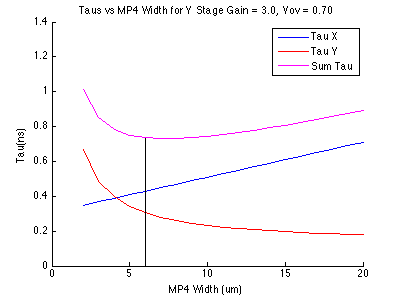
\includegraphics[width=10.63cm,height=7.99cm]{tau_x_y_vs_mp4.png}
\end{figure}


\begin{itemize}
\item MN6 is sized such that current through MN6 is same as the current 
through MP4 and MP5. 
\end{itemize}
$Id4=Id5=Id6=0.5\mu pCox(\frac{W4}{L4})(Vdd-Vx-abs(Vtp))^{2} (1+\lambda 
(Vdd-Vw)$\\


\begin{itemize}
\item Current through R3 and R4
\end{itemize}
$IR3+R4=Vss/(R3+R4)$\\




\begin{itemize}
\item $\tau stage2 (Vy)$
\end{itemize}
$=(R3 || R4)(Cgs7+Cgd7 (1+abs(A3))+Cgd6+Cdb6+Cgd5+Cdb5)$\\




\textbf{Stage 1}

\begin{itemize}
\item Vov4 from stage 2 sets Vx which in turn sets the ratio of R1 and 
R2.
\end{itemize}


$Vov4=Vdd-Vx-abs(Vtp) $\\


$x (\frac{R1}{R2})=\frac{Vdd}{Vx}-1 $\\


\begin{itemize}
\item Gain of stage 1 (Common gate amplifier) is set to 10000.
\end{itemize}
$abs(A1)=(R1 || R2) $\\


\begin{itemize}
\item MN1 and MP3 are sized such that Id1 = Id3.
\end{itemize}


\begin{itemize}
\item MN2 is sized to reduce Tau at n\_iin node. Tau (n\_iin) is 
inversely proportional to gm2.
\end{itemize}
$\tau stage1 (n_iin)=(\frac{1}{gm2})(Cin+Cgd1+Cdb1+Cgs2+Csb2)$\\


$\tau stage1 (Vx)=(R1 || R2)(Cgd2+Cbd2+Cgd3+Cdb3+Cgs4+Cgd4 (2))$\\




\begin{figure}[h]
\centering
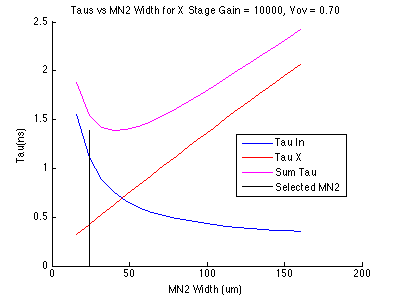
\includegraphics[width=10.63cm,height=7.99cm]{tau_i_x_vs_mn2.png}
\end{figure}


\begin{itemize}
\item Current through MN1, MN2 and MP3
\end{itemize}
$Id1,2,3=0.5\mu pCox(\frac{W3}{L3})(Vdd-VbiasP-abs(Vtp))^{2} (1+\lambda 
(Vdd-Vx))$\\


\begin{itemize}
\item Current through R1 and R2
\end{itemize}
$IR1+R2=Vdd/(R1+R2)$\\


\textbf{Vovn, Vovp}

\begin{itemize}
\item Vovn and Vovp are chosen to achieve a reasonable balance between 
gain, Tau total and Power.
\end{itemize}
$Gain total (A)=A1A2A3A4$\\


$\tau total=\tau stage1(n_{iin})+\tau stage1(Vx)+\tau stage2(Vy)+\tau 
stage3(Vz)+\tau stage1 (Vout)$\\


$
Power=(Vdd-Vss)(Id1+Id4+Id7+Id10)+(\frac{Vdd^{2}}{R1+R2})+(\frac{Vss^{2}}{R3+R4}) 
$\\


\begin{table}[h]
\centering
\begin{tabular}{|l|l|l|l|l|}
\hline
\textbf{Stage1} & Hand calculation & Spice & \%Error & Reason for 
error \\
\hline
Id1 &   &   &   &   \\
\hline
Vx &   &   &   &   \\
\hline
A1 (Gain of stage1) &   &   &   &   \\
\hline
gm2 &   &   &   &   \\
\hline
Tau (iin) &   &   &   &   \\
\hline
  &   &   &   &   \\
\hline
\textbf{Stage2} & Hand calculation & Spice & \%Error & Reason for 
error \\
\hline
Id4 &   &   &   &   \\
\hline
Vw &   &   &   &   \\
\hline
Vy &   &   &   &   \\
\hline
gm4 &   &   &   &   \\
\hline
A2 (Gain of stage2) &   &   &   &   \\
\hline
Tau (Vy) &   &   &   &   \\
\hline
  &   &   &   &   \\
\hline
\textbf{Stage3} & Hand calculation & Spice & \%Error & Reason for 
error \\
\hline
Id7 &   &   &   &   \\
\hline
Vz &   &   &   &   \\
\hline
gm7 &   &   &   &   \\
\hline
gm8 &   &   &   &   \\
\hline
A3 (Gain of stage3) &   &   &   &   \\
\hline
Tau (Vz) &   &   &   &   \\
\hline
  &   &   &   &   \\
\hline
\textbf{Stage4} & Hand calculation & Spice & \%Error & Reason for 
error \\
\hline
Id10 &   &   &   &   \\
\hline
Vout &   &   &   &   \\
\hline
Vt10 &   &   &   &   \\
\hline
gm10 &   &   &   &   \\
\hline
gmb10 &   &   &   &   \\
\hline
A4 (Gain of stage4) &   &   &   &   \\
\hline
Tau (vout) &   &   &   &   \\
\hline
  &   &   &   &   \\
\hline
Total Power &   &   &   &   \\
\hline
Total Gain &   &   &   &   \\
\hline
\end{tabular}
\end{table}

\pagebreak

%%%%%%%%%%%%%%%%%%%%%%%%%%%%%%%%%%%%%%%%%%%%%%%%%%%%%%%%%%%%%%%%%%%%%%%%%%%%%%%%
% Bode Diagrams - Page 7

% Simulated Bode Plots of A(jw), magnitude and phase. Clearly annotate the
% achieved gain and bandwidth. Annotate your hand-calculated values in the same
% plots, noting any specific features of interest (either from the results
% themselves or based on what you've learned in hand calculations or scripting
% the design). Plots must be annotated with meaningful comments/observations.

\section{Simulated Bode Plots}

\centering
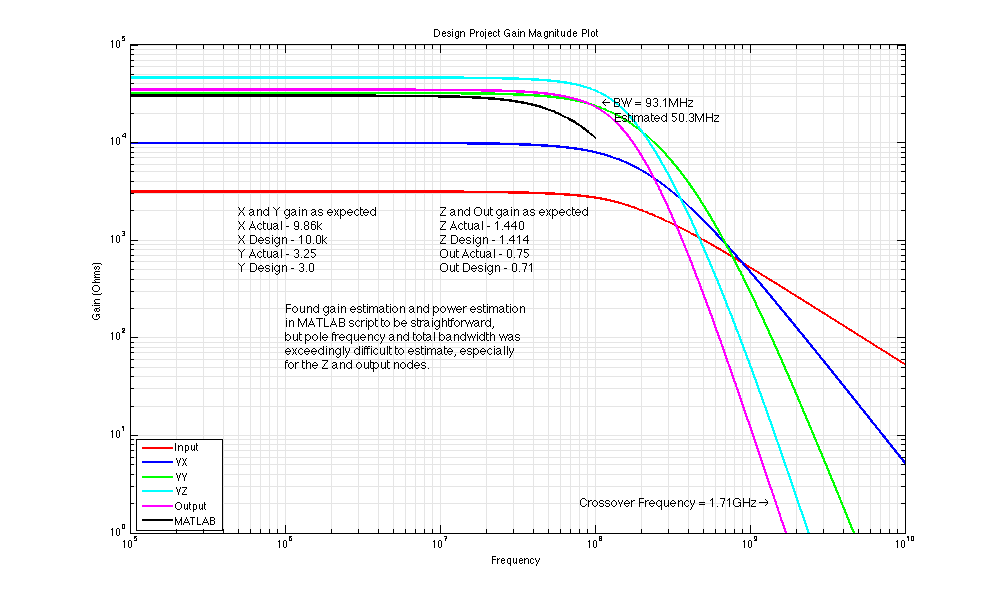
\includegraphics[width=\textwidth]{mag.png}

\centering
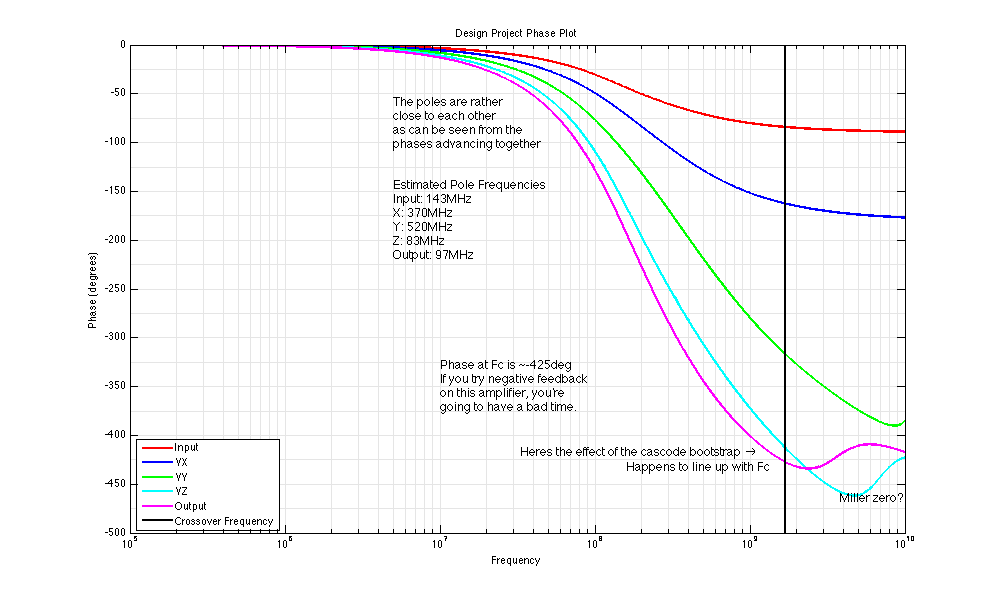
\includegraphics[width=\textwidth]{phase.png}

\pagebreak

%%%%%%%%%%%%%%%%%%%%%%%%%%%%%%%%%%%%%%%%%%%%%%%%%%%%%%%%%%%%%%%%%%%%%%%%%%%%%%%%
% Transient Response - Page 8

% Show a transient simulation plot of the output for a 1 MHz, 1 µA sinusoidal
% input current. Make sure that there is no distortion.

\section{Simulated Transient Response}
\begin{figure}[h]
\centering
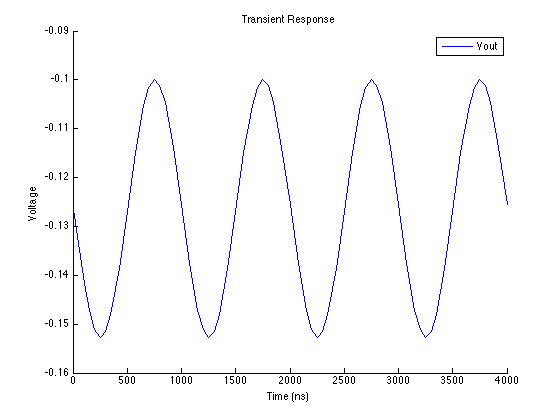
\includegraphics[scale=.75]{transient_response.png}
\end{figure}

\pagebreak


%%%%%%%%%%%%%%%%%%%%%%%%%%%%%%%%%%%%%%%%%%%%%%%%%%%%%%%%%%%%%%%%%%%%%%%%%%%%%%%%
% Comments and Conclusions - Page 9

% Comments and conclusion. Here, you can convey issues you may have had, or
% things you have learned/not learned in this project.

\section{Comments and Conclusion}


\begin{itemize}
\item Resistors contribute to a large part of the overall gain. From 
manufacturability perspective, passive components are not friendly and 
also occupy more area on the chip.
\item The output source follower stage is very sensitive to biasing due 
to back gate effect. Small variations on Vz can drive the output to fall 
out of desired common mode voltage or drive MN10 into cutoff region and 
lose all the gain from previous stages.
\item Any variations in supply voltage causes variation in Vov of MN7 
directly (as the device is biased through R3 \& R4) causing Vz to vary 
and thereby impacting the biasing of MN10 and gain.
\item Common source stage with diode connected load attributes to miller 
cap loading effect on cascade stage. This is limiting the gain of common 
source stage to smaller values.
\item Since the output is single ended, it is susceptible to noise. 
Differential configuration will be better.
\end{itemize}

\pagebreak

%%%%%%%%%%%%%%%%%%%%%%%%%%%%%%%%%%%%%%%%%%%%%%%%%%%%%%%%%%%%%%%%%%%%%%%%%%%%%%%%
% Spice Netlist - Appendix I

% Final SPICE netlist and .op output. Include only the MOSFET and node voltage
% listing from the .op output.

\section{Appendix I}
Netlist here

\end{document}
